 The bar graph representing the above data is shown in figure \ref{fig:bar38_py}\\
\begin{figure}[!ht]
\centering
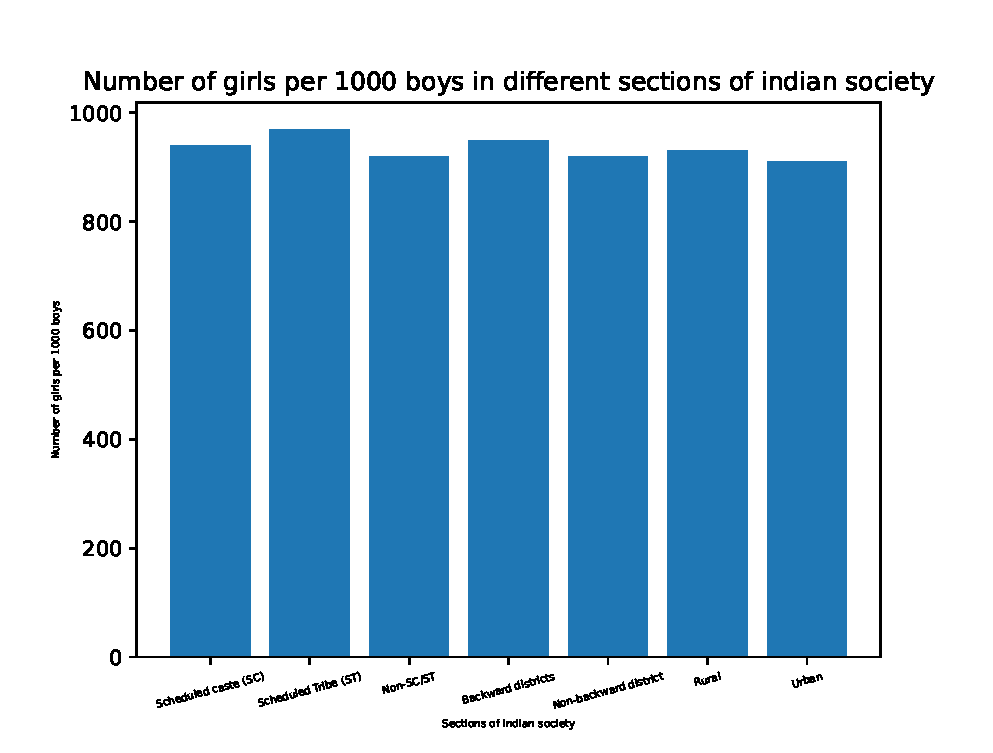
\includegraphics[width=\columnwidth]{./solutions/20-10/stat/codes/pyfigs/exer38.eps}
\caption{Number of girls per 1000 boys}
\label{fig:bar38_py}
\end{figure}
The python code for the above problem is 
\begin{lstlisting}
./solutions/20-10/stat/codes/exer38.py
\end{lstlisting}
